\chapter{Relativistic Quantum Field Theory}
In non-relativistic quantum mechanics
\begin{align*}
   E &= \frac{\pmb{p}^2}{2m} \\
   E &\mapsto i\hbar \frac{\partial}{\partial t} \\
   \pmb{p} &\rightarrow -i\hbar \pmb{\nabla}
\end{align*}

After promoting the momentum and energy into operators in dispersion relation we have the Schrödinger equation
\begin{align}
   i \frac{\partial}{\partial t} \psi + \frac{1}{2m} \pmb{\nabla}^2 \psi = 0
\end{align}

Density of probability is defined via
\begin{align}
   \rho = |\psi|^2 = \psi \psi^*
\end{align}
It obeys the continuity equation
\begin{align}
   -\frac{\partial}{\partial t } \int_V \rho \dd{V} &= \int \pmb{j} \cdot \pmb{n} \dd{S} \notag\\
                                                    &= \int_V \pmb{\nabla} \cdot \pmb{j} \dd{V} \notag \\
   \Rightarrow \frac{\partial \rho}{\partial t} + \div \pmb{j} &= 0
\end{align}

Writing this explicitly
\begin{align}
   \frac{\partial \rho}{\partial t} &= \frac{\partial }{\partial t} \left( \psi \psi^* \right) \notag\\
                                    &= \psi \frac{\partial \psi^*}{\partial t} + \psi^* \frac{\partial \psi}{\partial t} \notag \\
                                    &= \frac{i}{2m} \left( \psi^* \pmb{\nabla}^2 \psi -  \psi \pmb{\nabla}^2 \psi \right) \notag \\
   \Rightarrow \pmb{j} &= - \frac{i}{2m} \left( \psi^* \pmb{\nabla}^2 \psi -  \psi \pmb{\nabla}^2 \psi \right)
\end{align}

If we have a plane wave state, as an example 
\begin{align*}
   \psi &= N \euler^{i\pmb{p}\cdot \pmb{x} - i Et} \\
   \pmb{j} &= \frac{\pmb{p}}{m} |N|^2
\end{align*}

\section{Relativistic wave equation}
Now we enter the relativistic regime
\begin{align*}
   E^2 &= \pmb{p}^2 + m^2 \\
   p^\mu &= (E, \pmb{p}) \quad p_\mu = (E, -\pmb{p}) \\
   p^2 &= m^2
\end{align*}

Promoting energy and momentum into operators
\begin{align*}
   p^\mu &\mapsto i \partial^\mu \\
   \partial_\mu \partial^\mu &= \frac{\partial ^2}{\partial^2 t} - \nabla^2
\end{align*}

We have then Klein-Gordon equation
\begin{align}
   (\partial_\mu \partial^\mu + m^2) \phi(\pmb{x}, t) = 0
\end{align}

The current in KG-theory is conserved as well
\begin{align}
   j^\mu &= (\rho, \pmb{j}) = i \left( \phi^* \partial^\mu \phi - \phi \partial^\mu \phi^* \right) \\
   \partial_\mu j^\mu &= 0
\end{align}

An example solution
\begin{align*}
   \phi = N \euler^{-ip\cdot x} \\
   j^\mu = 2 p^\mu |N|^2
\end{align*}

In terms of Lorentz transformation
\begin{align*}
   \rho \sim E
\end{align*}

Energies of particles
\begin{align*}
   E^2 = \pmb{p}^2 + m^2 \\
   E = \pm \sqrt{\pmb{p}^2 + m^2}
\end{align*}

It also implies negative probability
\begin{align*}
   E > 0 \mapsto \rho > 0 \\
   E < 0 \mapsto \rho < 0
\end{align*}

\section{Feynman-Stückelberg Interpretation of negative energy states}
"Electron" with $E, \pmb{p}$ and charge $-e$
\begin{align*}
   j^\mu_{e^-} = 2e|N|^2(E,\pmb{p})
\end{align*}
"Positron" with $E, \pmb{p}$ and charge $+e$
\begin{align*}
   j^\mu_{e^+} = 2e|N|^2(E,\pmb{p})
   = - 2e|N|^2(-E,-\pmb{p})
\end{align*}

We can think of $E<0$ solution as particle flying backwards in time or $E > 0$ anti-particle forwards in time.
\begin{figure}[ht]
   \centering
   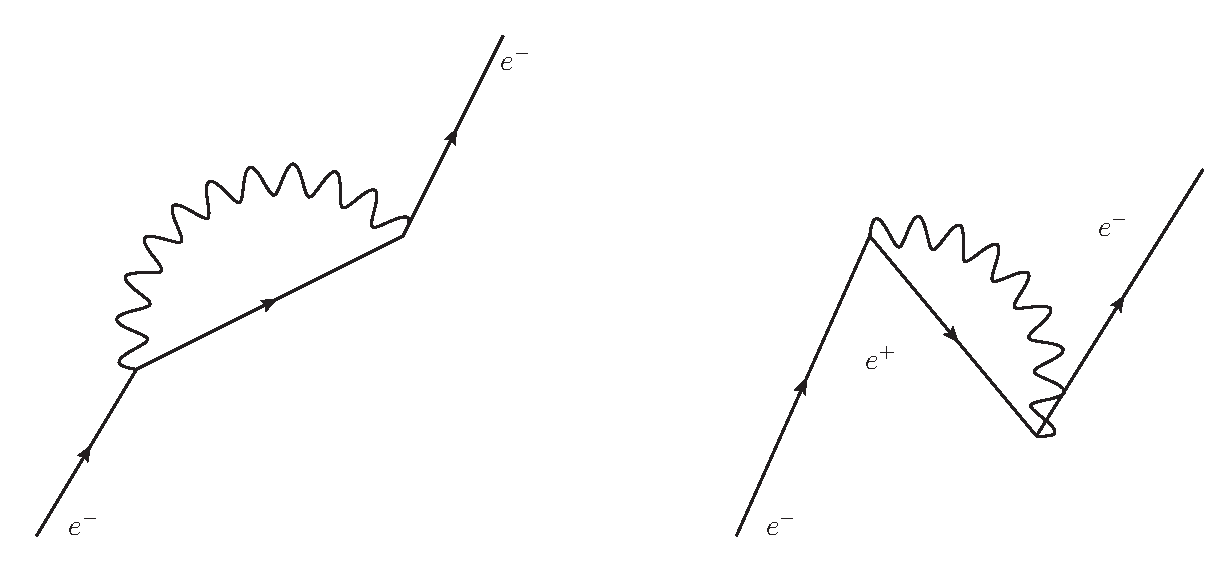
\includegraphics[width=0.8\linewidth]{fs-interpretation/fs-interpretation.eps}
   \caption{scattering process; horizontal time-axis; in the second diagram a electron positron pair is produced}%
   \label{fig:}
\end{figure}

In a relativistic systems we need to remember following points
\begin{itemize}
   \item anti-particles
   \item particle numbers are not conserved
\end{itemize}

\section{Electrodynamics (spin $1$)}
Maxwell equations are
\begin{align}
   \pmb{E} &= -\vec{\nabla} \phi - \frac{\dd}{\dd{t}}{\pmb{A}} \\
   \pmb{B} &= \vec{\nabla} \times \pmb{A}\\
   \vec{\nabla} \times \pmb{E} &= -\frac{\dd}{\dd{t}}{\pmb{B}} \\
   \div \pmb{B} &= 0
\end{align}

Field strength tensor and four-potential
\begin{align}
   F_{\mu\nu} &= \partial_\mu A_\nu - \partial_\nu A_\mu \\
   A^\mu(x) &= (\phi, \pmb{A})
\end{align}
The fields can be calculated from it
\begin{align}
   E^i &= F^{0i} = \partial^i A^0 - \partial ^0 A^i \\
   B_i &= -\epsilon_{ijk} \partial^i A^k = -\epsilon_{0ijk}F^{jk}
\end{align}

Often it is useful to use the dual tensor
\begin{align}
   \tilde{F}_{\mu\nu} &= \epsilon_{\mu\nu\sigma\tau} F^{\sigma \tau} \\
   \partial^{\mu} \tilde{F}_{\mu\nu} &= 0
\end{align}
is the second set of maxwell equations.

The other set of two equations is 
\begin{align}
   \partial_\nu F^{\mu\nu} = 4\pi j^\mu
\end{align}

$\pmb{E}, \pmb{B}$ are observable, $\pmb{A}$ is not. $A^\mu$ is not uniquely fixed by $\pmb{E}$ and $\pmb{B}$. It has the following gauge symmetry
\begin{align}
   \tilde{A}_{\mu} = A_\mu + \partial_\mu \Lambda(\pmb{x}, t)
\end{align}

Use this transformation to get
\begin{align}
   \partial_\mu A^\mu = 0
\end{align}

Plugging it back then we have the relativistic wave equation
\begin{align}
   \partial_\mu \partial^\mu A^\nu = 0
\end{align}
it essentially is Klein-Gordon equation with mass $m=0$

$A^\mu$ is a vector with spin $1$
\begin{align*}
   (j_+, j_-) = \left( \frac{1}{2}, \frac{1}{2} \right)
\end{align*}
It implied it has two transverse degrees of freedom. It has spin $1$ properties: $+1$, $0$, $-1$, in which $0$ mode does not exist.

\section{Description of Fermions}
Original motivation for Dirac. He wants a linear equation in $E$ or $\frac{\partial}{\partial t}$
\begin{align*}
   p^\mu \mapsto i\partial^\mu
\end{align*}

Take the ansatz
\begin{align*}
   i\hbar \frac{\partial}{\partial t}\psi &= H \psi \\
   &= (\vec{\alpha}\cdot \pmb{p} + \beta m ) \psi
\end{align*}
but $\pmb{\alpha}$ and $\beta$ unknown. It still has to obey the relativistic energy relation
\begin{align*}
   A &= \left( \alpha_ip_i + \beta m \right) \left( \alpha_ip_i + \beta m \right) \\
     &\stackrel{!}{=} \pmb{p}^2 + m^2 \\
     &= \alpha_i \alpha_j p_i p_j + \beta^2m^2 + \alpha_i \beta p_i m + \beta \alpha_j p_j m
\end{align*}

From this we demand
\begin{align}
   \beta^2 = 1 \\
   \alpha_i^2 = 1 \\
   \alpha_i \alpha_j + \alpha_j \alpha_i = 0 \\
   \alpha_i \beta + \beta \alpha_i = 0
\end{align}
So $\alpha$ and $\beta$ are not just numbers, but (can be proven to be) hermitian traceless matrices with eigenvalue $\pm 1$.  In addition, it only exits in even dimensions.
Since $\alpha_i$ and $\beta$ are $4\times4$ matrices. $\psi$ has to be a 4-component spinor.

For parity conservation need $(\frac{1}{2}, 0) \bigoplus (0, \frac{1}{2})$
Thus 
\begin{align*}
   \begin{pmatrix} \begin{pmatrix} & \\ & \end{pmatrix}_{2\times2} & \\ & \begin{pmatrix} & \\ &  \end{pmatrix}_{2\times2}   \end{pmatrix}
\end{align*}

There are different sets of $\alpha_i, \beta$ which satisfy the conditions. They are called representations.

Dirac-Pauli representation
\begin{align}
   \alpha_i &= \begin{pmatrix} 0 & \sigma^i \\ \sigma^i &  0 \end{pmatrix} \\
   \beta &= \begin{pmatrix} \id_2 & 0 \\ 0 & -\id_2\end{pmatrix}
\end{align}
with $\sigma^i$ the Pauli matrices.

Weyl (chiral) representation
\begin{align}
   \alpha^i &= \begin{pmatrix} -\sigma^i & 0 \\ 0 & \sigma^i \end{pmatrix}  \\
   \beta &= \begin{pmatrix} 0 & \id_2 \\ \id_2 & 0 \end{pmatrix}
\end{align}
they are mainly used in high energy physics (E $\gg m$).

\subsection{Gamma Matrices}
We now define 4 gamma matrices $\gamma^\mu$, $\mu=0,1,2,3$
\begin{align}
   \gamma^\mu = \left(\beta, \beta \pmb{\alpha} \right)
\end{align}
Note that having an index does not make it Lorentz vector.

The Clifford algebra is defined as following
\begin{align}
   \left\{ \gamma^\mu, \gamma^\nu \right\} = \gamma^\mu \gamma^\nu + \gamma^\nu \gamma^\mu = 2 g^{\mu\nu}
\end{align}

In Dirac-Pauli representation
\begin{align}
   \gamma^0 &= \begin{pmatrix} \id & 0 \\ 0 & -\id \end{pmatrix} \\
   \gamma^i &= \begin{pmatrix} 0 & \sigma^i \\ -\sigma^i & 0 \end{pmatrix} \\
   \gamma^5 &= i \gamma^0 \gamma^1 \gamma^2 \gamma^3 = \begin{pmatrix} 0 & \id \\ \id & 0\end{pmatrix}
\end{align}

In Weyl representation 
\begin{align*}
   \gamma^0 \leftrightarrow \gamma^5
\end{align*}

Rewriting the Dirac equation using $\gamma$s
\begin{align}
   i \partial_t \psi &= \left( \pmb{\alpha} \cdot \pmb{p} + \beta m  \right) \psi \notag\\
   i \partial_t \psi &= -i \pmb{\alpha} \cdot \vec{\nabla} \psi + m \beta \psi \notag\\
   i \beta \partial_t \psi &= -i \beta \pmb{\alpha} \cdot \vec{\nabla} \psi + m \psi \notag\\
   \left(i\gamma^\mu \partial_\mu - m \right) \psi &= 0
\end{align}
Conventionally we use $\phi$ for spin $0$ particle and $A_\mu$ for spin $1$.

It is convenient to also have an equation for $\psi^\dagger$. First one can show $\gamma^\mu^\dagger = \gamma^0 \gamma^\mu \gamma^0$.
\begin{itemize}
   \item $\mu = 0$: $\gamma^0 = \beta$ and $\gamma^0^\dagger = \gamma^0 \gamma^0 \gamma^0$ $\Rightarrow \beta^2 = \id_4$
   \item $\gamma^\mu^\dagger = (\beta \alpha^k)^\dagger = (\alpha^k)^\dagger \beta^\dagger = \alpha^k \beta = \beta^2 \alpha^k \beta = \beta \gamma^k \beta = \gamma^0 \gamma^k \gamma^0$
\end{itemize}

\begin{align}
   i \gamma^0 \partial_0 \psi + i \gamma^k \partial_k \partial - m \psi = 0 \notag\\
   -i \partial_0 \psi^\dagger (\gamma^0)^\dagger - i(\partial_k \psi^\dagger) \gamma^k^\dagger - m \psi^\dagger = 0 \notag \\
   -i \partial_0 \psi^\dagger \gamma^0 - i(\partial_k \psi^\dagger) \gamma^0 \gamma^k \gamma^0 - m \psi^\dagger = 0 \notag \\
   \shortintertext{define $\bar{\psi} = \psi^\dagger \gamma^0$}
   -i \partial_0 \bar{\psi} \gamma^0 - i \partial_\mu \bar{\psi} \gamma^\mu - m \bar{\psi} = 0 \notag \\
   i(\partial_\mu \bar{\psi}) \gamma^\mu + m \bar{\psi} = 0
\end{align}

\subsection{Free Particle Solution to Dirac Equation}
\begin{align*}
   \left( i \gamma^\mu \partial_\mu - m \right) \psi &= 0 \\
   \shortintertext{multiplying $\gamma^\nu \partial_\nu$ from left}
   i\gamma^\mu \gamma^\nu \partial_\mu \partial_\nu \psi - m \gamma^\nu \partial_\nu \psi &= 0 \\
   i \gamma^\mu \gamma^\nu \partial_\mu \partial_\nu \psi + i m^2 \psi &= 0 \\
\end{align*}

\begin{align*}
   \gamma^\mu \gamma^\nu  &= \frac{1}{2} \left( \gamma^\mu \gamma^\nu + \gamma^\nu \gamma^\mu  \right) \\
                          &= \frac{1}{2} \left( \gamma^\mu \gamma^\nu - \gamma^\nu \gamma^\mu + 2g^{\mu\nu} \right) \\
                          &= \frac{1}{2} \left[ \gamma^\mu , \gamma^\nu \right] + g^{\mu\nu}
\end{align*}
The commutator is anti-symmetric and multiplying to symmetric tensor (derivatives) the term must vanish.

Each component of spinor satisfies the Klein-Gordon equation.
\begin{align}
   (\partial_\mu \partial^\mu + m^2) \psi_i = 0
\end{align}

Thus we can write the solution as plane-wave
\begin{align}
   \psi = u(\pmb{p}) \euler^{-ipx}
\end{align}
$u(\pmb{p})$ is also a 4-component object but as function $\pmb{p}$ not $\pmb{x}$

Insert in back into Dirac equation, then we have Dirac equation in momentum space
\begin{align}
   \left( \gamma^\mu p_\mu - m \right) u(\pmb{u}) = 0
\end{align}

Solution by considering Dirac-Pauli representation
\begin{align*}
   \left( \slashed{p} - m \right) u(\pmb{p}) = \begin{pmatrix} (E-m) \id & - \pmb{p} \cdot \pmb{\sigma} \\ \pmb{p} \cdot \pmb{\sigma} & -(E+m) \id \end{pmatrix} 
   \begin{pmatrix} u_A \\ u_B\end{pmatrix}
\end{align*}

$\pmb{p} = 0$ then $E = \pm m$

\begin{itemize}
   \item $E = +m$ Two solutions 
      \begin{align*}
         u_B = \begin{pmatrix} 1 \\ 0 \end{pmatrix} , \begin{pmatrix} 0 \\ 1\end{pmatrix}
      \end{align*}

   \item $E=-m$
      \begin{align*}
         u_A = \begin{pmatrix} 1 \\ 0\end{pmatrix}, \begin{pmatrix} 0 \\ 1\end{pmatrix}
      \end{align*}
\end{itemize}

$\pmb{p} = 0$
\begin{align}
   \pmb{\sigma} \cdot \pmb{p} u_B &= (E-m) u_A \\
   \pmb{\sigma} \cdot \pmb{p} u_A &= (E+m) u_B
\end{align}

\begin{itemize}
   \item $E>0$ 
      \begin{align*}
         \chi^{(1)} &= \begin{pmatrix} 1 \\ 0\end{pmatrix} \\
         \chi^{(2)} &= \begin{pmatrix} 0 \\ 1\end{pmatrix}
      \end{align*}
\end{itemize}

Ansatz $u_A^{(s)} = \chi^{(s)}$
\begin{align}
   u_B^{(s)} = \frac{\pmb{\sigma}\cdot\pmb{p}}{E + m} &\quad u_A^{(s)} = \frac{\pmb{\sigma}\cdot\pmb{p}}{E + m} \chi^{(s)} \notag\\
   u(\pmb{p}) &= N \begin{pmatrix} \chi^{(s)} \\ \frac{\pmb{\sigma}\cdot\pmb{p}}{E + m} \chi^{(s)}\end{pmatrix}
\end{align}

$E < 0$ and $u_B^{(s)} = \chi^{(s)}$
\begin{align}
   u(\pmb{p}) = N \begin{pmatrix} -\frac{\pmb{\sigma}\cdot\pmb{p}}{E + m} \chi^{(s)} \\ \chi^{(s)}\end{pmatrix}
\end{align}

One can show $u^{(r)}^\dagger u^{(s)} = N^2 \delta^{rs}$

Two fold degeneracy in each case. $ \begin{pmatrix} 1 \\ 0\end{pmatrix}$ and $ \begin{pmatrix} 0 \\ 1\end{pmatrix} $ for $E > 0$ and $E < 0$. There must be another observable which commutes with $H$ and $\pmb{p}$.
\begin{align*}
   H = \gamma^i p_i + \gamma^0 m
\end{align*}
\begin{align}
   \pmb{S} \cdot \hat{P} = \frac{1}{2} \begin{pmatrix} \pmb{\sigma}\cdot\pmb{p} & 0 \\ 0 & \pmb{\sigma}\cdot \hat{p}\end{pmatrix}
\end{align}

Helicity
\begin{align}
   \frac{1}{2} \pmb{\sigma} \cdot \hat{\hat{p}} &= \frac{1}{2} \begin{pmatrix} \hat{p}_z & \hat{p}_x + i\hat{p}_y \\ \hat{p}_x -i \hat{p}_y & -\hat{p}_z\end{pmatrix} \\
   \det(\pmb{\sigma} \cdot \hat{p}) &= - \hat{p}^2 = - 1
\end{align}
  
Determinant is the product of two eigenvalues, then
\begin{align*}
   \lambda_1 + \lambda_2 = 0 \\
   \lambda_1 \cdot \lambda_2 = 1 \\
   \lambda_{1,2} = \pm 1
\end{align*}

Antiparticle solution $u^{(3,4)}(-\pmb{p}) e^{-i(-p)x} = v^{(2,1)}$
\begin{align}
   \left( \slashed{p} + m \right)v(\pmb{p}) = 0
\end{align}

Normalization is
\begin{align}
   \int \rho \dd{V} = 2E \\
   N = \sqrt{E+m}
\end{align}

Completeness relation (spin sums)
\begin{align}
   \sum u^{(s)}(p) \bar{u}^{(s)}(p ) = \left( \slashed{p} + m \right) \\
   \sum v^{(s)}(p) \bar{v}^{(s)}(p ) = \left( \slashed{p} - m \right)
\end{align}

Define a projector projecting out positive and negative energy states
\begin{align}
   \Lambda_{\pm} = \frac{\pm \slashed{p} + m}{2m}
\end{align}

In Chiral (Weyl) representation
\begin{align}
   \left( \slashed{p} - m \right) u(\pmb{p}) = \begin{pmatrix} m & p \cdot \sigma \\ \vecp \cdot \bar{\sigma} & -m \end{pmatrix} \begin{pmatrix} u_L \\ u_R\end{pmatrix}
\end{align}
$\bar{\sigma} = (\sigma^0 , -\pmb{\sigma})$ and $\sigma^0 = \id_2$

Weyl equation
\begin{align}
   -m u_L + p\cdot \sigma u_R = 0 \\
   p \cdot \bar{\sigma} u_L - m u_R = 0
\end{align}
if $m=0$, the equations decouple.

